\documentclass[11pt]{article}

\usepackage{titling,lipsum,hyperref}
\usepackage[margin=1in]{geometry}
\usepackage{graphicx,amsmath,hyperref}
\usepackage[english]{babel}
\usepackage[utf8]{inputenc}
\usepackage{fancyhdr}

\newenvironment{localsize}[1]
{%
  \clearpage
  \let\orignewcommand\newcommand
  \let\newcommand\renewcommand
  \makeatletter
  \input{bk#1.clo}%
  \makeatother
  \let\newcommand\orignewcommand
}
{%
  \clearpage
}

\pagestyle{fancy}
\fancyhf{}
\rhead{ENGN3100 Report}
\lhead{Uri Pierre Burmester (u5561093)}
\rfoot{Page \thepage}

\title{ENGN3100 Practical Experience Report}
\author{Uri Pierre Burmester (u5561093)}
\date{\today}

\begin{document}

\begin{figure} \centering
  
\includegraphics[width=0.5\linewidth]{ANU.png}
\end{figure}

\maketitle

\centerline{AUSTRALIAN NATIONAL UNIVERSITY}  
\centerline{College of Engineering and Computer Science} 

\bigskip

\centerline{This Report is submitted in partial fulfilment of the Requirements for Practical Experience}
\centerline{ for the BE Degree in the ANU College of Engineering \& Computer Science}

\newpage

\tableofcontents

\newpage

\section{Summary of Practical Experience}

Period 1: \\
Name of Employer: Advanced Instrumentation and Technology Centre (RSAA) \\
Starting date of Employment: 20/11/2017 \\
Ending date of Employment: 19/01/2018 \\
Position/job: Summer Research Intern - High-altitude Balloon Project \\
Weeks of experience claimed: 8 \\

\medskip

Period 2: \\
Name of Employer: Questacon - The National Science and Technology Centre \\
Starting date of Employment: 01/08/2017 \\
Ending date of Employment: 19/11/2017 \\
Position/job: Gallery Assistant \\
Weeks of experience claimed: 4 \\

Total number of weeks of experience claimed: 12

\newpage

\section{Letters of Employment / Declaration of IEAUST requirements}
\subsection{AITC Letter}

\begin{figure}[!h] \centering
  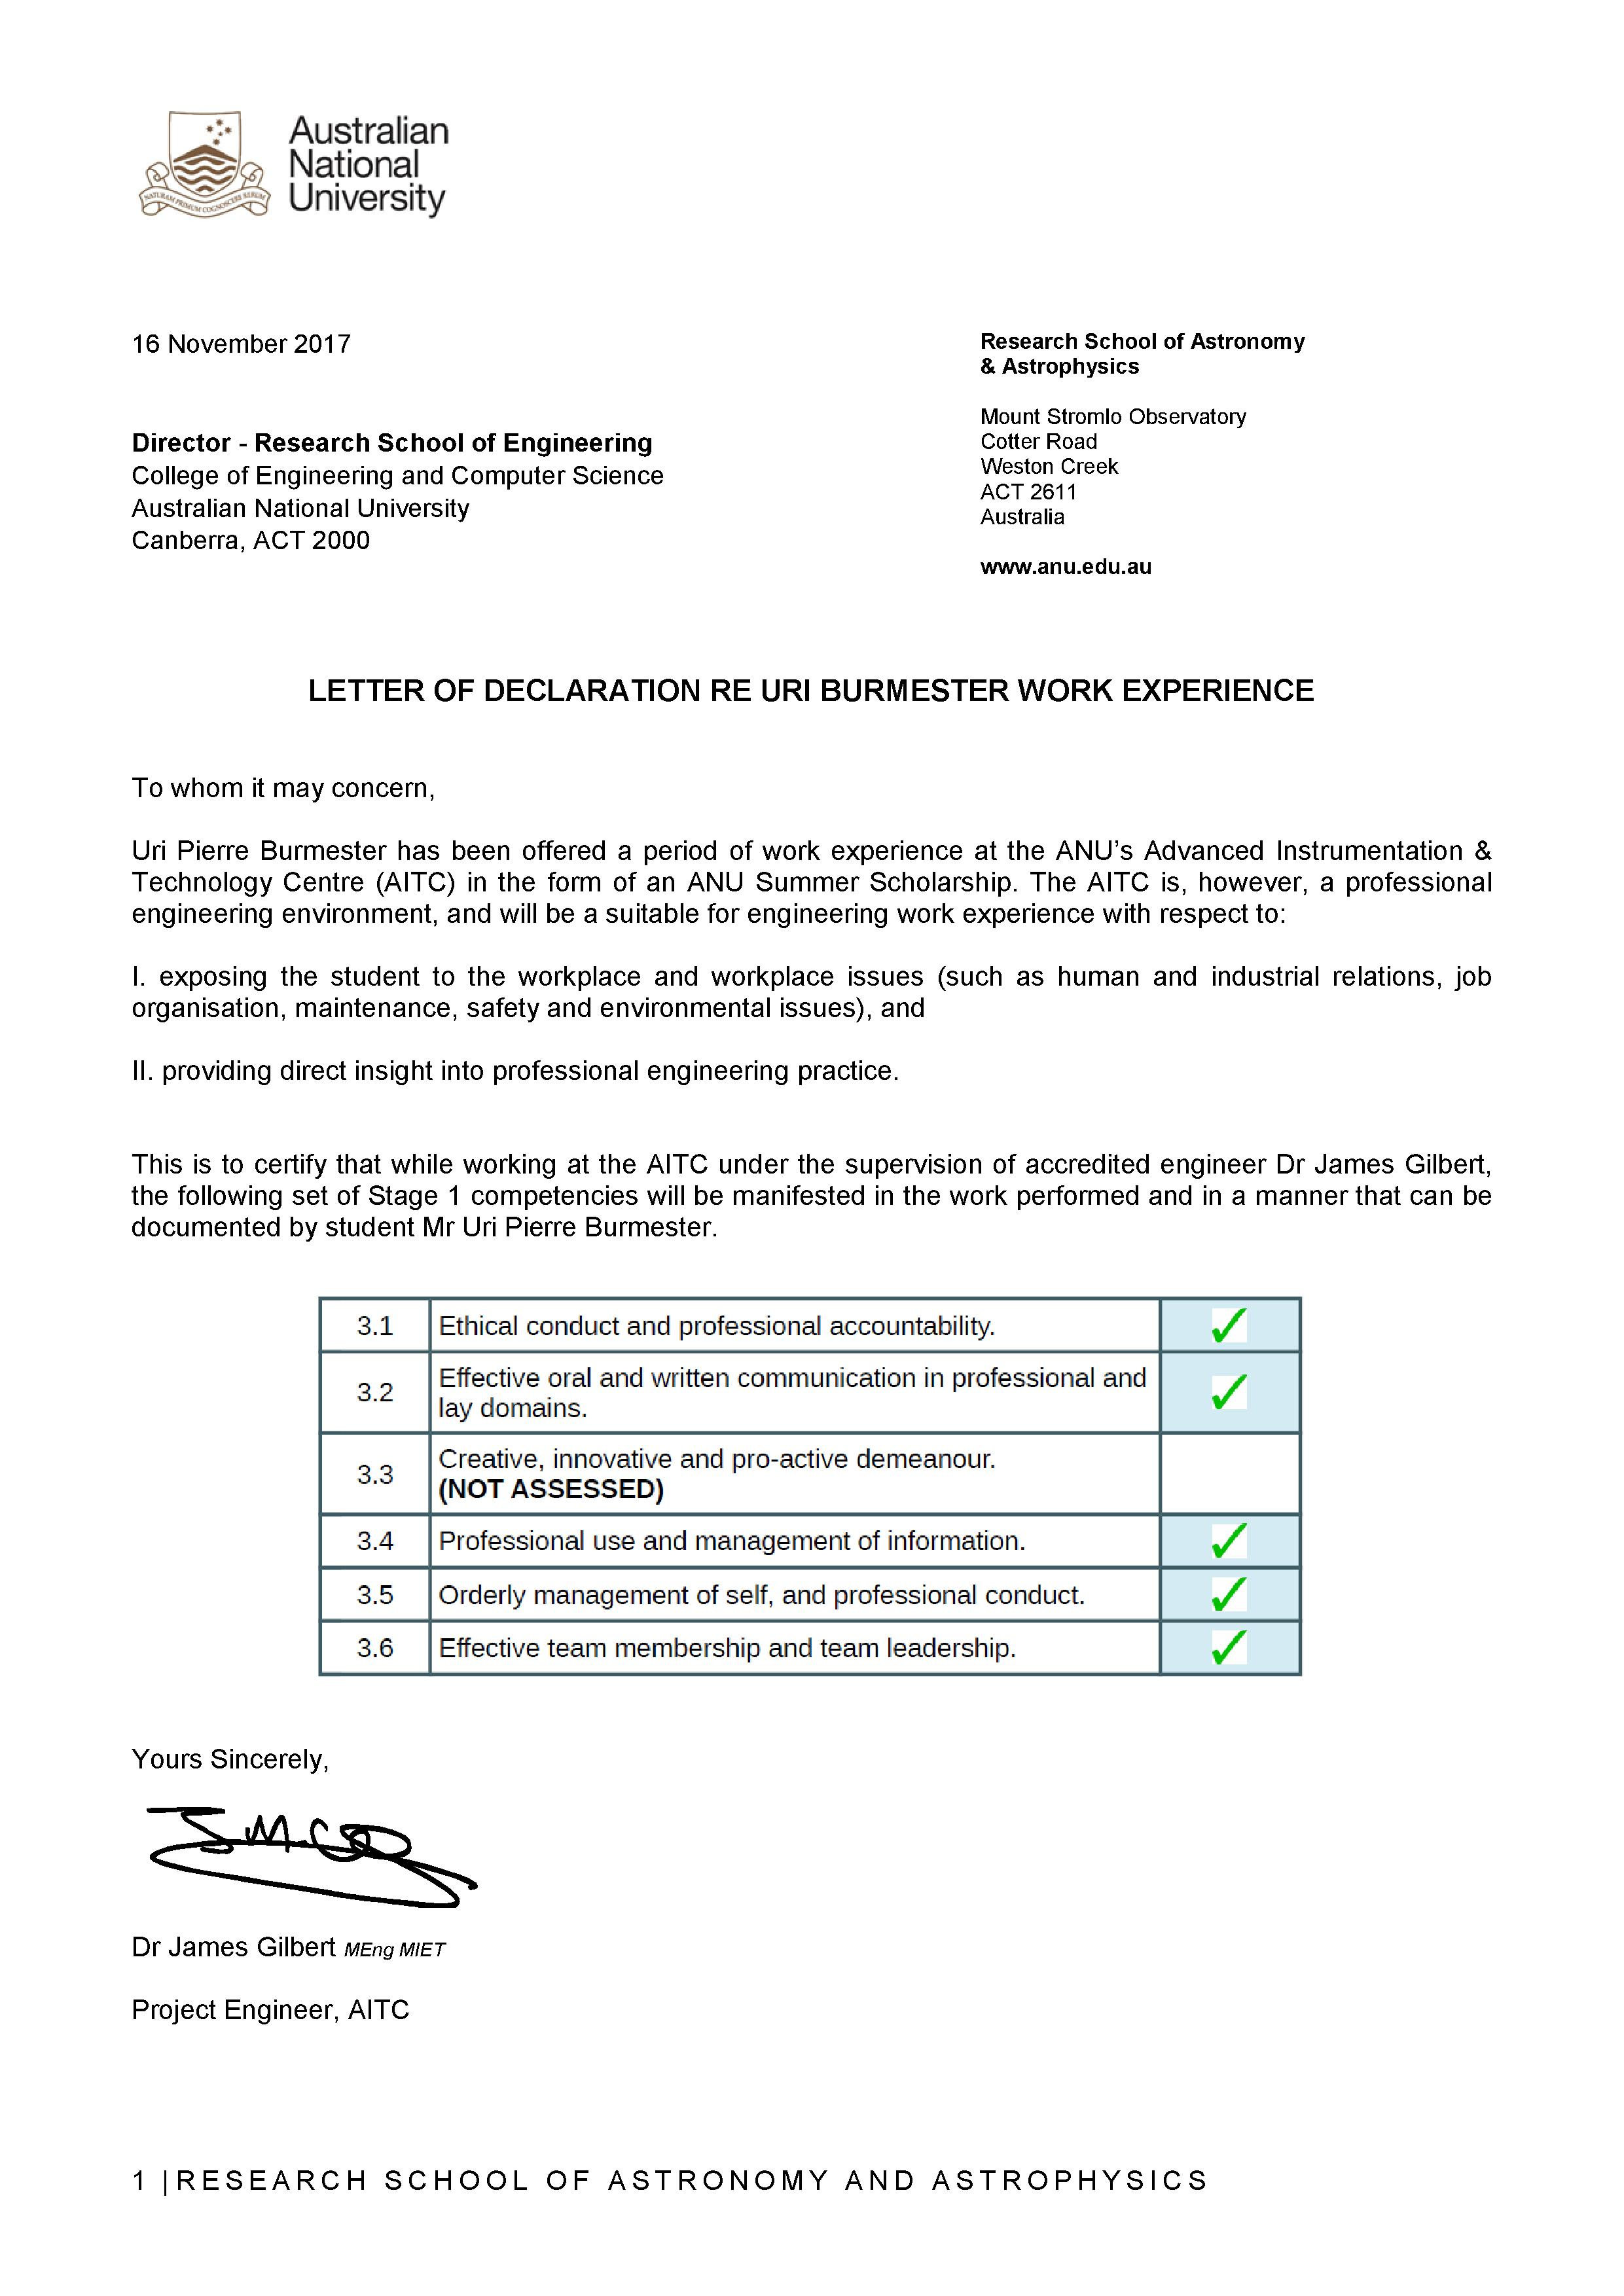
\includegraphics[width=0.89\linewidth]{upb_offer-signed.jpg}
\end{figure}

\newpage

\subsection{Questacon Letter}

SIGNED LETTER OF EMPLOYMENT FROM QUESTACON

\newpage

\section{Report}

\subsection{AITC Report}

\subsubsection{The structure and operation of the Company}
-3-4 pages

- Advanced Instrumentation and Technology Centre, run by the ANU's Research School of Astronomy and Astrophysics
Mount Stromlo Obervatory
Weston ACT 2611
%T +61 2 6125 0230, %E aitc@anu.edu.au, %W aitc.anu.edu.au



- Company's full name, associates, parent or autonomous?
- Company head-quarters full address, telephone, Internet, etc.
- Managerial and administrative structure of the company.
- Company's business/ products, production output, trading partners, markets.
- Company's divisions (if there are any). Division's business/products, etc.
- Name and address of the Head of the Division.
- Company's financial base, is it private or public, is it listed on Stock Exchange?
- Total operation budget, division into business areas.
- Attitude of the company to its work-force, prevailing ethics in the company.

\subsubsection{My Position in the Company}
-1-2 pages

- Title of my job/ jobs.
- My immediate supervisor, and my position within the structure.
- Responsibility and requirements in my job(s).
- Interaction with other employees.
- Why was the job offered to me?

\subsubsection{Technical Description of the Job}
-5-6 pages
- What I did (attach summary results as appendix, if relevant).
- What I achieved (attach any drawings, photographs, sketches as appendix, if
relevant).
- How did my work relate to Company's business?

\subsection{Questacon Report}

This report does not include my experiences at Questacon because, as stated in the requirements on the \href{http://programsandcourses.anu.edu.au/course/engn3100}{ENGN3100 course page}: "The report itself need only describe the experience at one of the places (must be one of the places satisfying the engineering requirement)."

\newpage

\section{Development of Stage 1 Competency Standards for Professional Engineer}

-2-3 pages
- How my experiences helped me work towards the standards of a
professional engineer.
- The standards identified by Engineers Australia are listed on the ENGN3100
WebCT report site
- Which areas of competency were developed, and how.\
PLEASE NUMBER EACH COMPETENCY CLAIMED ACCORDING TO THE
NUMBERING SYSTEM OF APPENDIX 1.

\newpage

\section{Employer Feedback Forms}

\subsection{AITC}

EMPLOYER FEEDBACK FORM FROM AITC

\newpage

\subsection{Questacon}

EMPLOYER FEEDBACK FORM FROM QUESTACON

\newpage

\section{Employer Declarations of Report Accuracy}

\subsection{AITC}

EMPLOYER DECLARATION FROM AITC

\newpage

\subsection{Questacon}

EMPLOYER DECLARATION FROM QUESTACON

\newpage

\section{Conclusions}
-1 page

\newpage

\section{Reflection of Work Experience}
-1 page

\newpage

\section{Acknowledgements}

-Jamie
-Jess Brosnan

\section{Signature and date}

\medskip

Signature: .................................................................................................. \\
Date: \today

\newpage

\section{Appendix 1: Stage 1 Competency Matrix}
\begin{localsize}{10}

\begin{table} \centering
 \begin{tabular}{|p{0.75cm} | p{8cm} | p{1.5cm} | p{2.5cm} | p{2.5cm}|} 
 \hline
  Unit & UNIT Descriptor & Claimed? [Y/N] & Section or Line or Paragraph where covered in Report & Line-numbers where covered in Journal\\ [0.5ex] \hline
   1 & KNOWLEDGE AND SKILL BASE & & & \\ \hline
   1.1 & Comprehensive, theory based understanding of the underpinning natural and physical sciences and the engineering fundamentals applicable to the engineering discipline. & & & \\ \hline
   1.2 & Conceptual understanding of the, mathematics, numerical analysis, statistics, and computer and information sciences which underpin the engineering discipline. & & & \\ \hline
   1.3 & In-depth understanding of specialist bodies of knowledge within the engineering discipline. & & & \\ \hline
   1.4 & Discernment of knowledge development and research directions within the
engineering discipline. & & & \\ \hline
   1.5 & Knowledge of contextual factors impacting the
engineering discipline. & & & \\ \hline
   1.6 & Understanding of the scope, principles, norms, accountabilities and bounds of contemporary engineering practice in the specific discipline. & & & \\ \hline
   & & & & \\ \hline
   2 & ENGINEERING APPLICATION ABILITY & & & \\ \hline
   2.1 & Application of established engineering methods to complex engineering problem solving. & & & \\ \hline
   2.2 & Fluent application of engineering techniques, tools and resources. & & & \\ \hline
   2.3 & Application of systematic engineering synthesis and design processes & & & \\ \hline
   2.4 & Application of systematic approaches to the conduct and management of engineering projects. & & & \\ \hline
   & & & & \\ \hline
   3 & PROFESSIONAL AND PERSONAL ATTRIBUTES & & & \\ \hline
   3.1 & Ethical conduct and professional accountability & & & \\ \hline
   3.2 & Effective oral and written communication in professional and lay domains & & & \\ \hline
   3.3 & Creative, innovative and pro-active demeanour. & & & \\ \hline
   3.4 & Professional use and management of information. & & & \\ \hline
   3.5 & Orderly management of self, and professional conduct. & & & \\ \hline
   3.6 & Effective team membership and team leadership. & & & \\ \hline
   \end{tabular}
\caption{Australian Engineering Competency Standards, Engineers Australia
Competencies for Stage 1 Engineering Practitioners}
\end{table}

\end{localsize}

\end{document}